\documentclass{article}

\usepackage{fancyhdr}
\usepackage{extramarks}
\usepackage{amsmath}
\usepackage{amsthm}
\usepackage{amsfonts}
\usepackage{tikz}
\usepackage[plain]{algorithm}
\usepackage{algpseudocode}
\usepackage{listings}
\usepackage{caption}
\usepackage{tabularray}

\usepackage{graphicx}

\usepackage{hyperref}

\usepackage{cleveref}
\usetikzlibrary{automata,positioning}

%
% Basic Document Settings
%

\topmargin=-0.45in
\evensidemargin=0in
\oddsidemargin=0in
\textwidth=6.5in
\textheight=9.0in
\headsep=0.25in

\linespread{1.1}

\pagestyle{fancy}
\lhead{\hmwkAuthorName}
\chead{\hmwkClass: \hmwkTitle}
\rhead{\firstxmark}
\lfoot{\lastxmark}
\cfoot{\thepage}

\renewcommand\headrulewidth{0.4pt}
\renewcommand\footrulewidth{0.4pt}

\setlength\parindent{0pt}

%
% Create Problem Sections
%

\newcommand{\enterProblemHeader}[1]{
    \nobreak\extramarks{}{Task \arabic{#1} continued on next page\ldots}\nobreak{}
    \nobreak\extramarks{Task \arabic{#1} (continued)}{Task \arabic{#1} continued on next page\ldots}\nobreak{}
}

\newcommand{\exitProblemHeader}[1]{
    \nobreak\extramarks{Task \arabic{#1} (continued)}{Task \arabic{#1} continued on next page\ldots}\nobreak{}
    \stepcounter{#1}
    \nobreak\extramarks{Task \arabic{#1}}{}\nobreak{}
}

\setcounter{secnumdepth}{0}
\newcounter{partCounter}
\newcounter{homeworkProblemCounter}
\setcounter{homeworkProblemCounter}{1}
\nobreak\extramarks{Task \arabic{homeworkProblemCounter}}{}\nobreak{}

%
% Homework Problem Environment
%
% This environment takes an optional argument. When given, it will adjust the
% problem counter. This is useful for when the problems given for your
% assignment aren't sequential. See the last 3 problems of this template for an
% example.
%
\newenvironment{homeworkProblem}[1][-1]{
    \ifnum#1>0
        \setcounter{homeworkProblemCounter}{#1}
    \fi
    \section{Task \arabic{homeworkProblemCounter}}
    \setcounter{partCounter}{1}
    \enterProblemHeader{homeworkProblemCounter}
}{
    \exitProblemHeader{homeworkProblemCounter}
}

%
% Homework Details
%   - Title
%   - Due date
%   - Class
%   - Section/Time
%   - Instructor
%   - Author
%

\newcommand{\hmwkTitle}{Homework\ \#1}
\newcommand{\hmwkDueDate}{September 30, 2024}
\newcommand{\hmwkClass}{Computational Photography}
\newcommand{\hmwkClassTime}{ }
\newcommand{\hmwkClassInstructor}{Professor Cho Sunghyun}
\newcommand{\hmwkAuthorName}{\textbf{Shipilova Polina}}

%
% Title Page
%

\title{
    \vspace{2in}
    \textmd{\textbf{\hmwkClass:\ \hmwkTitle}}\\
    \normalsize\vspace{0.1in}\small{Due\ on\ \hmwkDueDate\ }\\
    \vspace{0.1in}\large{\textit{\hmwkClassInstructor\ \hmwkClassTime}}
    \vspace{3in}
}

\author{\hmwkAuthorName}
\date{}

\renewcommand{\part}[1]{\textbf{\large Part \Alph{partCounter}}\stepcounter{partCounter}\\}

%
% Various Helper Commands
%

% Useful for algorithms
\newcommand{\alg}[1]{\textsc{\bfseries \footnotesize #1}}

% For derivatives
\newcommand{\deriv}[1]{\frac{\mathrm{d}}{\mathrm{d}x} (#1)}

% For partial derivatives
\newcommand{\pderiv}[2]{\frac{\partial}{\partial #1} (#2)}

% Integral dx
\newcommand{\dx}{\mathrm{d}x}

% Alias for the Solution section header
\newcommand{\solution}{\textbf{\large Solution}}

% Probability commands: Expectation, Variance, Covariance, Bias
\newcommand{\E}{\mathrm{E}}
\newcommand{\Var}{\mathrm{Var}}
\newcommand{\Cov}{\mathrm{Cov}}
\newcommand{\Bias}{\mathrm{Bias}}

\begin{document}

\maketitle

\pagebreak

\begin{homeworkProblem}
\subsubsection{GAUSSIAN FILTERING}

The main part of a code is $apply\_gaussian\_filter$ function. It has such parametrs as

 $image, kernel\_size, kernel\_sigma, border\_type, separable$. 

At first, we need to initialize image and check is it colored or gray-scaled. For colored image we apply filter for each color channel separately. For gray-scaled image we use filter only once. 

If the kernel is separable, the 2D filter can be expressed as the outer product of two 1D vectors. This reduces computational complexity since we can apply two 1D convolutions (one for rows and one for columns) instead of a full 2D convolution. A common way to check if a filter is separable is by using Singular Value Decomposition (SVD). If the rank of the matrix representing the 2D kernel is 1, it means the kernel is separable and can be written as the outer product of two vectors.

\begin{lstlisting}[language=Python]
	def check_separable(kernel):
	 u, s, vt = np.linalg.svd(kernel)
	
	# Check the number of non-zero singular values
	rank = np.sum(s > 1e-10) 
	
	# If the rank is 1, the filter is separable
	return rank == 1, u, s, vt
\end{lstlisting}


If filter can be separated we perform convolution for rows and columns separately. I use function pad from NumPy libruary. It pads an array with chosen numbers of elements and modes for borders could be as follows: ‘constant’, ‘edge’, ‘linear\_ramp’, ‘maximum’, ‘mean’, ‘median’, ‘minimum’, ‘reflect’, ‘symmetric’, ‘wrap’, ‘empty’. 

For inseparable filter we should use only one convolution between an image array and a filter kernel.

\begin{lstlisting}[language=Python]
	def convolve_2d(image, kernel, border_type):
	...
	
	# Pad the image to handle borders
	padded_image = np.pad(image, ((pad_h, pad_h), (pad_w, pad_w)), mode=border_type)
	
	# Create an empty output array
	result = np.zeros_like(image)
	
	# Perform convolution
	for i in range(image_h):
		for j in range(image_w):
			region = padded_image[i:i + kernel_h, j:j + kernel_w]
			result[i, j] = np.sum(region * kernel)
	return result
\end{lstlisting}

\begin{table}[h]
	\begin{tabular}{c}
		Here is an example for $kernel\_size = 5, sigma = 2, border\_type="constant"$.\\
		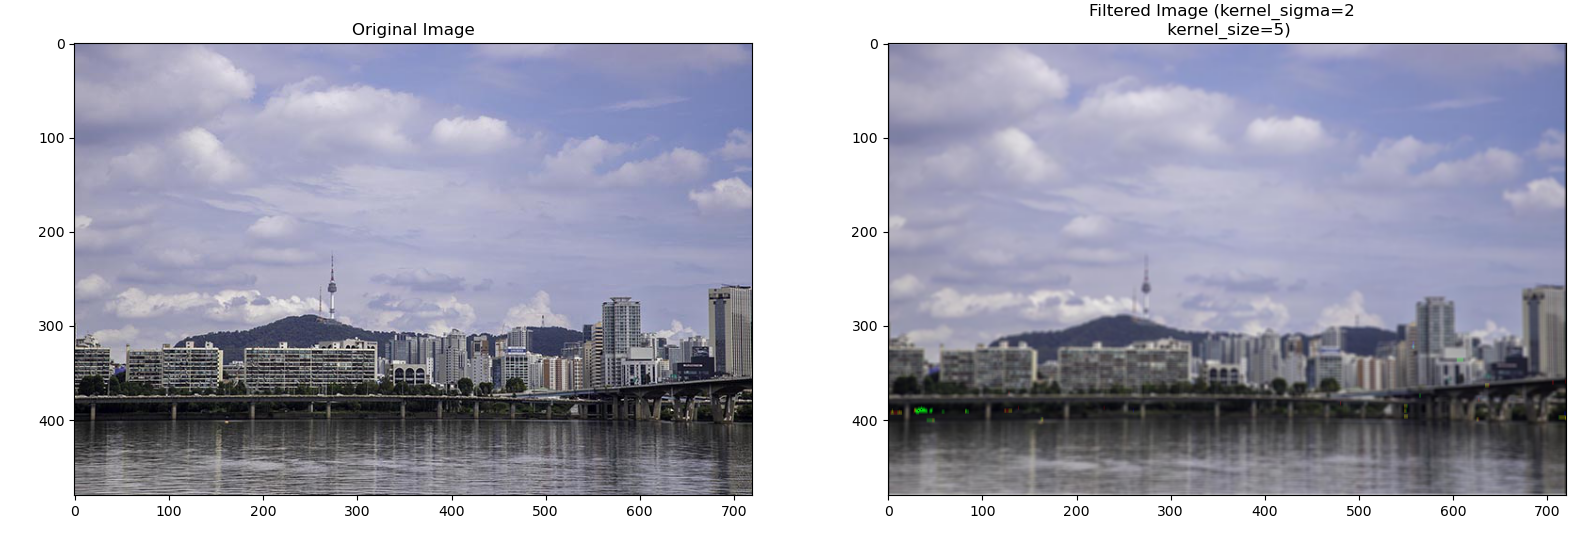
\includegraphics[totalheight=5cm]{images/g1}	\\
		Here is an example for $kernel\_size = 10, sigma = 5, border\_type="constant"$. \\ $kernel\_size$ should be set as $2-3sigma$ since it is a usual place to truncate Gaussian function. \\ According to the picture the more is sigma, the more picture is blurred.	\\
		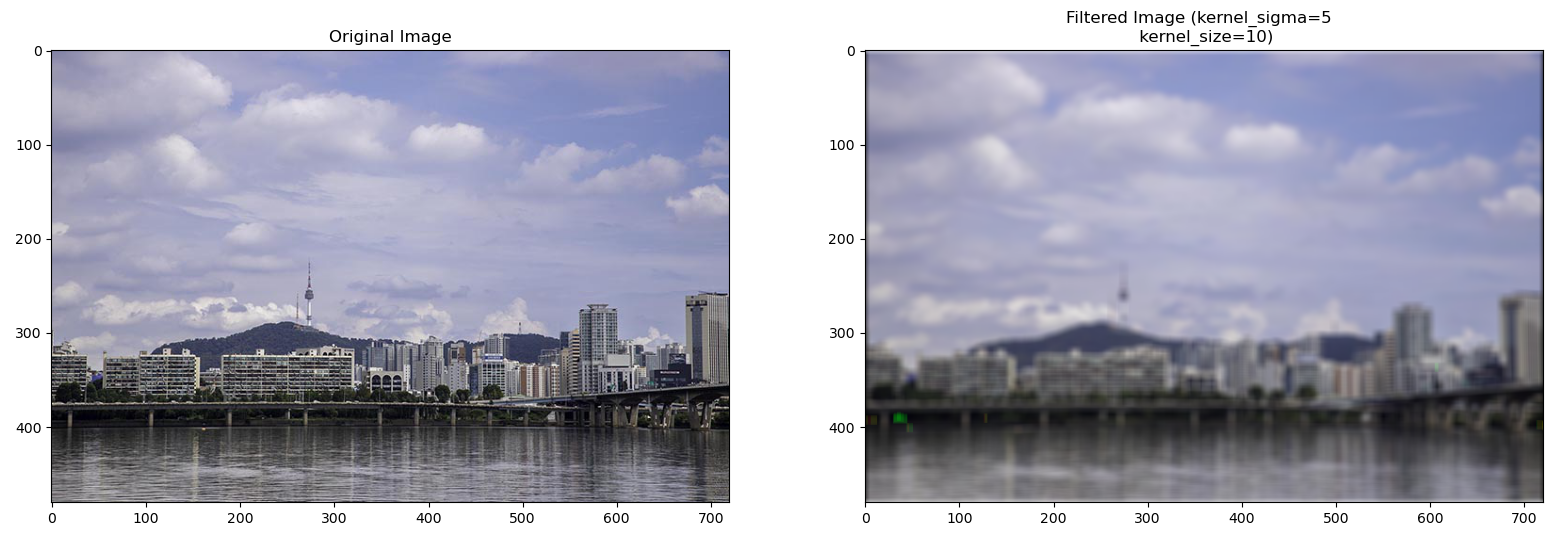
\includegraphics[totalheight=5cm]{images/g2}	\\
		
	\end{tabular}
\end{table}

\begin{table}
	\centering
	\begin{tblr}{
			vline{-} = {1}{},
			vline{1-2} = {2-4}{},
			hline{1-2} = {-}{},
			hline{3-5} = {1}{},
		}
		&  &  &  \\
		&  &  &  \\
		&  &  &  \\
		&  &  &  
	\end{tblr}
\end{table}

\end{homeworkProblem}
 
 
 
\pagebreak

\begin{homeworkProblem}
	\subsubsection{HISTOGRAM EQUALIZATION}
	
Before histogram equalization I load an image and divide colored one into tree different samples. After that I apply histogram calculation to flatten image. 
	\begin{lstlisting}[language=Python]
		histogram, _ = np.histogram(image_flat, bins=256, range=(0, 256))
	\end{lstlisting}
	    	
And calculate the cumulative distribution function (CDF) for histogram. Based on the result the CDF normalized to increase image contrast. At the end the original pixel values mapped to equalized values.

Here is my example:

\begin{table}[h]
	\begin{tabular}{c}
	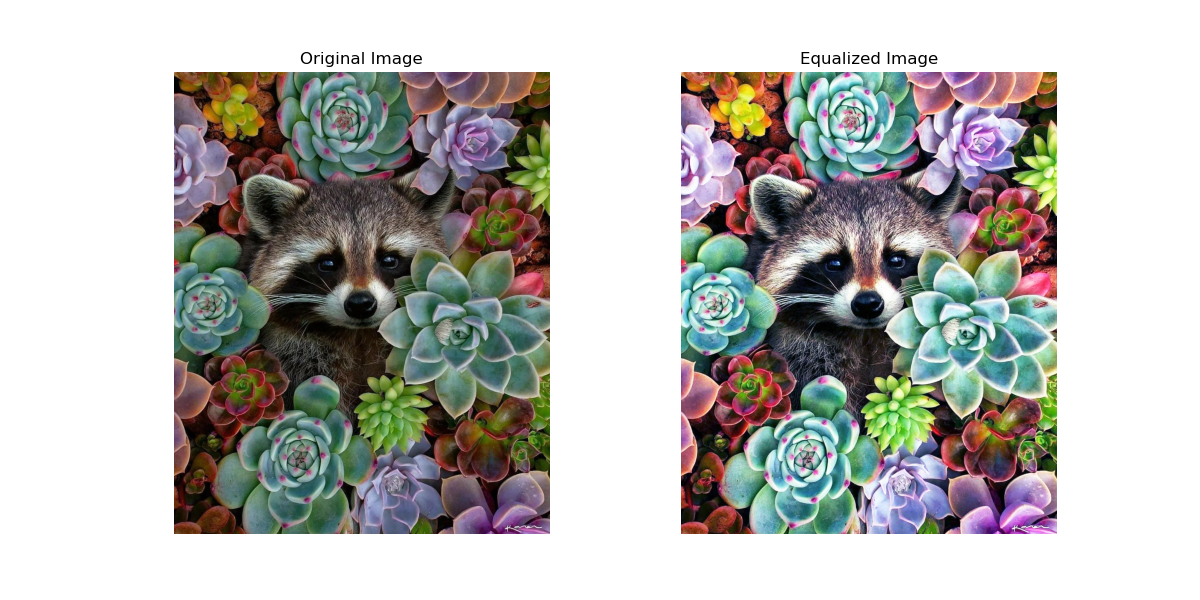
\includegraphics[totalheight=7cm]{images/example1}	\\
	With this colorful image histogram equalization works well. Colors became more bright and difference \\ between  the darkest and the lightest parts became bigger. Here we can't find a lot of artifacts, hence the \\ original picture haven't overexposed or underexposed parts. 	\\
	
	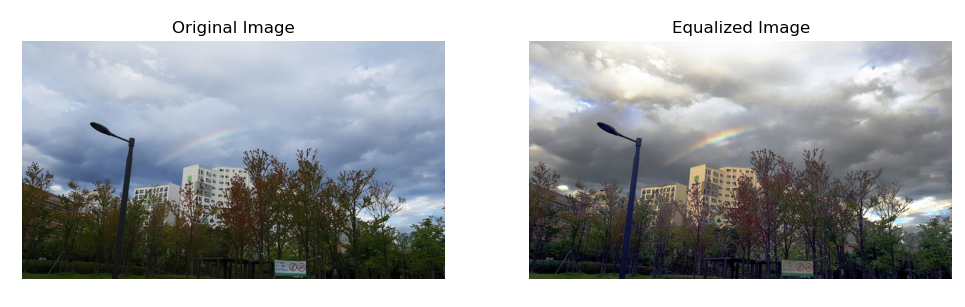
\includegraphics[totalheight=5cm]{images/exp1}	\\
	Here  we can see how blue sky became more gray, but the rainbow is brighter now.	
		
	\end{tabular}
\end{table}

\begin{table}[h]
	\begin{tabular}{c}
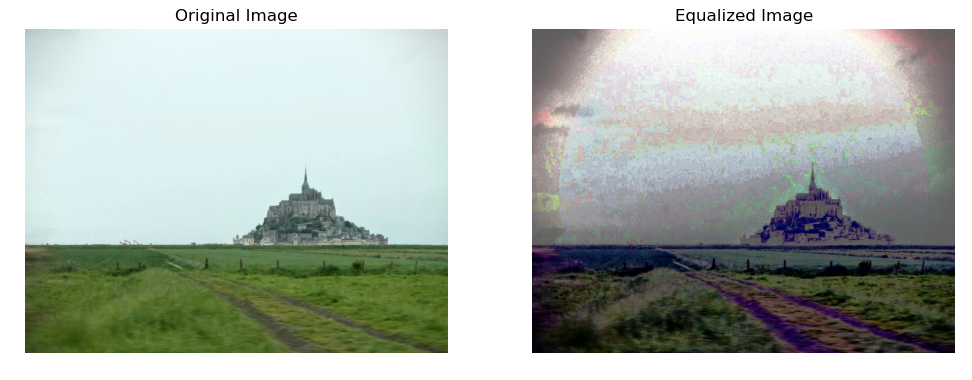
\includegraphics[totalheight=5cm]{images/exp2}	\\
Histogram equalization works really bad with this image. We can see a dirty sky after filtering. \\ I think that kind of artifacts appears due to the huge amount of white sky without any texture. 	\\
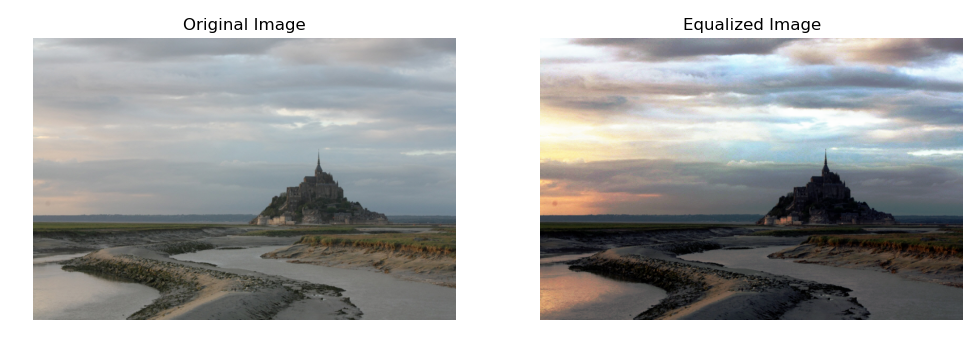
\includegraphics[totalheight=5cm]{images/exp3}	\\
On this picture  we can see how all the colors became more bright after enhancement. \\ The artifact here is a very dark regions on the ground and a castle.\\
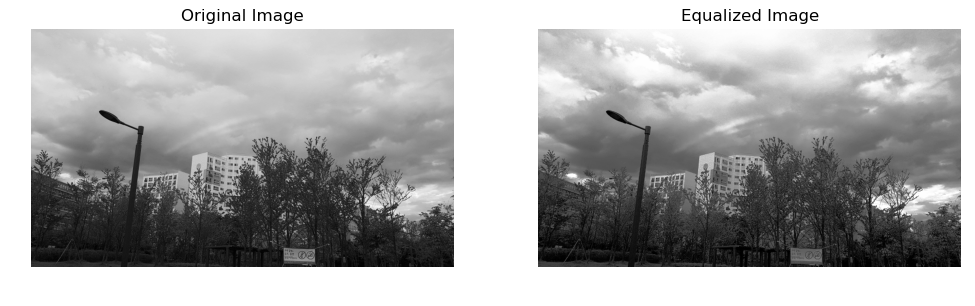
\includegraphics[totalheight=5cm]{images/exp4}	\\
This image  has become more even. In my opinion, the contrast has decreased and the light and dark \\ regions have become more uniform.	
	\end{tabular}
\end{table}


\begin{table}[h]
	\begin{tabular}{c}

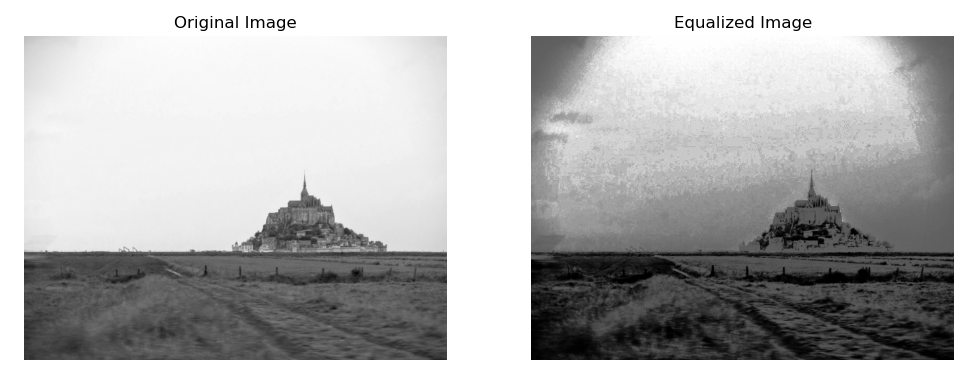
\includegraphics[totalheight=5cm]{images/exp5}	\\
With this picture  we have pretty similar problem that before with colored one. The white sky simply \\ became a mixture of different shades of gray.	\\
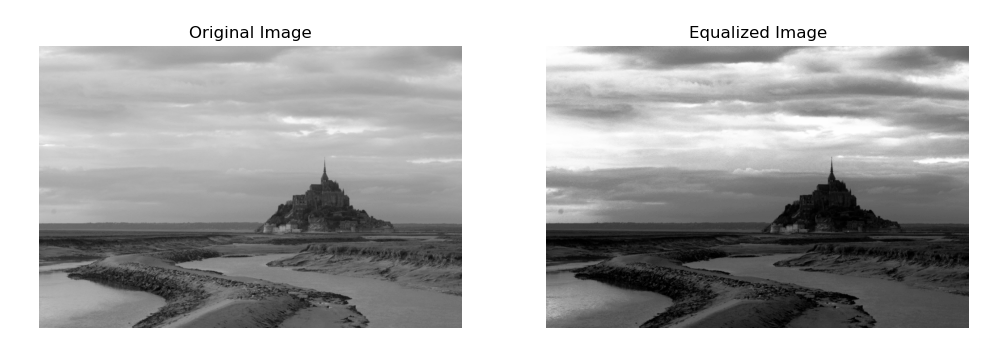
\includegraphics[totalheight=5cm]{images/exp6}	\\
Here you can see how much the contrast has increased. \\
\\
As a result, I want to say that histogram equalization method increases the contrast \\ of the image well and makes the colors more saturated. However, for more correct image\\  processing, we should not just normalize the histogram over the entire  region, but monitor the \\ original  image so as not to make the dark areas too black, and the already light areas too light. \\  Therefore, we should shift the histogram to those areas where there is no large peak.
	\end{tabular}
\end{table}


\pagebreak




	
\end{homeworkProblem}

\end{document}
